% Name: Venn diagram with elements
% Description: The numbers 1 to 12 sorted into the multiples of 2 and the multiples of 3, with 6 and 12 in the overlap and the rest outside both.
% Tags: venn, elements, sets, multiples

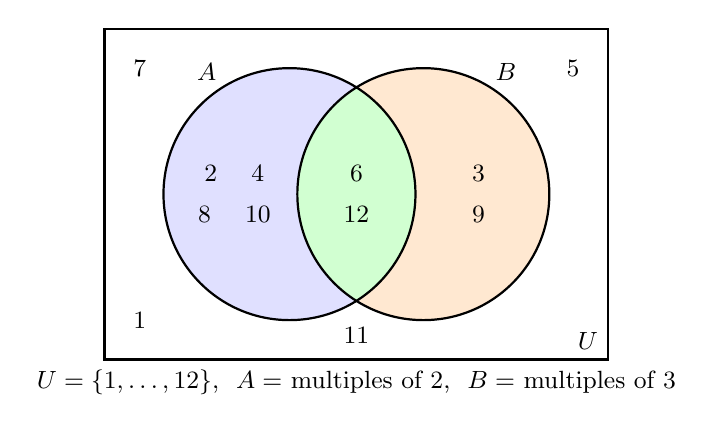
\begin{tikzpicture}[thick, every node/.style={font=\small}]
  \fill[blue!12] (-0.85,0) circle (1.6);
  \fill[orange!18] (0.85,0) circle (1.6);
  \begin{scope}
    \clip (-0.85,0) circle (1.6);
    \fill[green!18] (0.85,0) circle (1.6);
  \end{scope}
  \draw (-0.85,0) circle (1.6) (0.85,0) circle (1.6);
  \draw (-3.2,-2.1) rectangle (3.2,2.1);
  \node at (-1.9,1.55) {$A$};
  \node at (1.9,1.55) {$B$};
  \node[above left] at (3.2,-2.1) {$U$};
  \node[align=center] at (-1.55,0) {$2$ \quad $4$ \\[4pt] $8$ \quad $10$};
  \node[align=center] at (0,0) {$6$ \\[4pt] $12$};
  \node[align=center] at (1.55,0) {$3$ \\[4pt] $9$};
  \foreach \p/\n in {{(-2.75,-1.6)}/1, {(2.75,1.6)}/5, {(-2.75,1.6)}/7, {(0,-1.8)}/11} \node at \p {$\n$};
  \node[below, align=center] at (0,-2.1) {$U = \{1, \dots, 12\}$, \ $A = $ multiples of $2$, \ $B = $ multiples of $3$};
\end{tikzpicture}
